% Options for packages loaded elsewhere
\PassOptionsToPackage{unicode}{hyperref}
\PassOptionsToPackage{hyphens}{url}
%
\documentclass[
]{article}
\usepackage{lmodern}
\usepackage{amsmath}
\usepackage{ifxetex,ifluatex}
\ifnum 0\ifxetex 1\fi\ifluatex 1\fi=0 % if pdftex
  \usepackage[T1]{fontenc}
  \usepackage[utf8]{inputenc}
  \usepackage{textcomp} % provide euro and other symbols
  \usepackage{amssymb}
\else % if luatex or xetex
  \usepackage{unicode-math}
  \defaultfontfeatures{Scale=MatchLowercase}
  \defaultfontfeatures[\rmfamily]{Ligatures=TeX,Scale=1}
\fi
% Use upquote if available, for straight quotes in verbatim environments
\IfFileExists{upquote.sty}{\usepackage{upquote}}{}
\IfFileExists{microtype.sty}{% use microtype if available
  \usepackage[]{microtype}
  \UseMicrotypeSet[protrusion]{basicmath} % disable protrusion for tt fonts
}{}
\makeatletter
\@ifundefined{KOMAClassName}{% if non-KOMA class
  \IfFileExists{parskip.sty}{%
    \usepackage{parskip}
  }{% else
    \setlength{\parindent}{0pt}
    \setlength{\parskip}{6pt plus 2pt minus 1pt}}
}{% if KOMA class
  \KOMAoptions{parskip=half}}
\makeatother
\usepackage{xcolor}
\IfFileExists{xurl.sty}{\usepackage{xurl}}{} % add URL line breaks if available
\IfFileExists{bookmark.sty}{\usepackage{bookmark}}{\usepackage{hyperref}}
\hypersetup{
  pdftitle={markymark},
  pdfauthor={katherine piatti},
  hidelinks,
  pdfcreator={LaTeX via pandoc}}
\urlstyle{same} % disable monospaced font for URLs
\usepackage[margin=1in]{geometry}
\usepackage{color}
\usepackage{fancyvrb}
\newcommand{\VerbBar}{|}
\newcommand{\VERB}{\Verb[commandchars=\\\{\}]}
\DefineVerbatimEnvironment{Highlighting}{Verbatim}{commandchars=\\\{\}}
% Add ',fontsize=\small' for more characters per line
\usepackage{framed}
\definecolor{shadecolor}{RGB}{248,248,248}
\newenvironment{Shaded}{\begin{snugshade}}{\end{snugshade}}
\newcommand{\AlertTok}[1]{\textcolor[rgb]{0.94,0.16,0.16}{#1}}
\newcommand{\AnnotationTok}[1]{\textcolor[rgb]{0.56,0.35,0.01}{\textbf{\textit{#1}}}}
\newcommand{\AttributeTok}[1]{\textcolor[rgb]{0.77,0.63,0.00}{#1}}
\newcommand{\BaseNTok}[1]{\textcolor[rgb]{0.00,0.00,0.81}{#1}}
\newcommand{\BuiltInTok}[1]{#1}
\newcommand{\CharTok}[1]{\textcolor[rgb]{0.31,0.60,0.02}{#1}}
\newcommand{\CommentTok}[1]{\textcolor[rgb]{0.56,0.35,0.01}{\textit{#1}}}
\newcommand{\CommentVarTok}[1]{\textcolor[rgb]{0.56,0.35,0.01}{\textbf{\textit{#1}}}}
\newcommand{\ConstantTok}[1]{\textcolor[rgb]{0.00,0.00,0.00}{#1}}
\newcommand{\ControlFlowTok}[1]{\textcolor[rgb]{0.13,0.29,0.53}{\textbf{#1}}}
\newcommand{\DataTypeTok}[1]{\textcolor[rgb]{0.13,0.29,0.53}{#1}}
\newcommand{\DecValTok}[1]{\textcolor[rgb]{0.00,0.00,0.81}{#1}}
\newcommand{\DocumentationTok}[1]{\textcolor[rgb]{0.56,0.35,0.01}{\textbf{\textit{#1}}}}
\newcommand{\ErrorTok}[1]{\textcolor[rgb]{0.64,0.00,0.00}{\textbf{#1}}}
\newcommand{\ExtensionTok}[1]{#1}
\newcommand{\FloatTok}[1]{\textcolor[rgb]{0.00,0.00,0.81}{#1}}
\newcommand{\FunctionTok}[1]{\textcolor[rgb]{0.00,0.00,0.00}{#1}}
\newcommand{\ImportTok}[1]{#1}
\newcommand{\InformationTok}[1]{\textcolor[rgb]{0.56,0.35,0.01}{\textbf{\textit{#1}}}}
\newcommand{\KeywordTok}[1]{\textcolor[rgb]{0.13,0.29,0.53}{\textbf{#1}}}
\newcommand{\NormalTok}[1]{#1}
\newcommand{\OperatorTok}[1]{\textcolor[rgb]{0.81,0.36,0.00}{\textbf{#1}}}
\newcommand{\OtherTok}[1]{\textcolor[rgb]{0.56,0.35,0.01}{#1}}
\newcommand{\PreprocessorTok}[1]{\textcolor[rgb]{0.56,0.35,0.01}{\textit{#1}}}
\newcommand{\RegionMarkerTok}[1]{#1}
\newcommand{\SpecialCharTok}[1]{\textcolor[rgb]{0.00,0.00,0.00}{#1}}
\newcommand{\SpecialStringTok}[1]{\textcolor[rgb]{0.31,0.60,0.02}{#1}}
\newcommand{\StringTok}[1]{\textcolor[rgb]{0.31,0.60,0.02}{#1}}
\newcommand{\VariableTok}[1]{\textcolor[rgb]{0.00,0.00,0.00}{#1}}
\newcommand{\VerbatimStringTok}[1]{\textcolor[rgb]{0.31,0.60,0.02}{#1}}
\newcommand{\WarningTok}[1]{\textcolor[rgb]{0.56,0.35,0.01}{\textbf{\textit{#1}}}}
\usepackage{graphicx}
\makeatletter
\def\maxwidth{\ifdim\Gin@nat@width>\linewidth\linewidth\else\Gin@nat@width\fi}
\def\maxheight{\ifdim\Gin@nat@height>\textheight\textheight\else\Gin@nat@height\fi}
\makeatother
% Scale images if necessary, so that they will not overflow the page
% margins by default, and it is still possible to overwrite the defaults
% using explicit options in \includegraphics[width, height, ...]{}
\setkeys{Gin}{width=\maxwidth,height=\maxheight,keepaspectratio}
% Set default figure placement to htbp
\makeatletter
\def\fps@figure{htbp}
\makeatother
\setlength{\emergencystretch}{3em} % prevent overfull lines
\providecommand{\tightlist}{%
  \setlength{\itemsep}{0pt}\setlength{\parskip}{0pt}}
\setcounter{secnumdepth}{-\maxdimen} % remove section numbering
\ifluatex
  \usepackage{selnolig}  % disable illegal ligatures
\fi

\title{markymark}
\author{katherine piatti}
\date{2/7/2021}

\begin{document}
\maketitle

R markdown documents are good for creating sharable reports of you work.
to generate the report from this markdown file click the knit button at
the top.

\hypertarget{headings}{%
\section{Headings}\label{headings}}

to create headings, subheadings, and sub-sub headings, etc. use hashes

\hypertarget{heading-1}{%
\section{Heading 1}\label{heading-1}}

\hypertarget{heading-2}{%
\subsection{Heading 2}\label{heading-2}}

\hypertarget{heading-3}{%
\subsubsection{Heading 3}\label{heading-3}}

\hypertarget{heading-4}{%
\subsubsection{Heading 4}\label{heading-4}}

make sure to add a space after the hashes.

\hypertarget{bold-and-italics}{%
\section{bold and italics}\label{bold-and-italics}}

you can make text bold and ital using astricks.

\textbf{i want to make this bold} \emph{i want to make this italics}

\hypertarget{bullets}{%
\section{bullets}\label{bullets}}

to add bullet points use dashes.

\begin{itemize}
\tightlist
\item
  bullet 1
\item
  bullet 2
\item
  bullet 3
\end{itemize}

don't forget to put a space after the dash.

\hypertarget{quotes}{%
\section{quotes}\label{quotes}}

to make nicely formatted quotations use \textgreater{}

\begin{quote}
``there definitely are stupid questions.'' -katherine piatti, rladies
sydney learner
\end{quote}

\hypertarget{links}{%
\section{links}\label{links}}

to add links to you report put text label for link in square brackets
and url in round brakets.
\href{https://rladiessydney.org/courses/ryouwithme/04-markymark-1/}{here}
is the link.

\hypertarget{picturesgifstweets}{%
\section{pictures/gifs/tweets}\label{picturesgifstweets}}

you can easily add additional types of content to your markdown report.

\hypertarget{pictures}{%
\subsubsection{pictures}\label{pictures}}

the image file needs to be in the same .proj directory as your markdown
file. use square brackets for the label you want on the image. put the
image file name in round brackets.

\begin{figure}
\centering
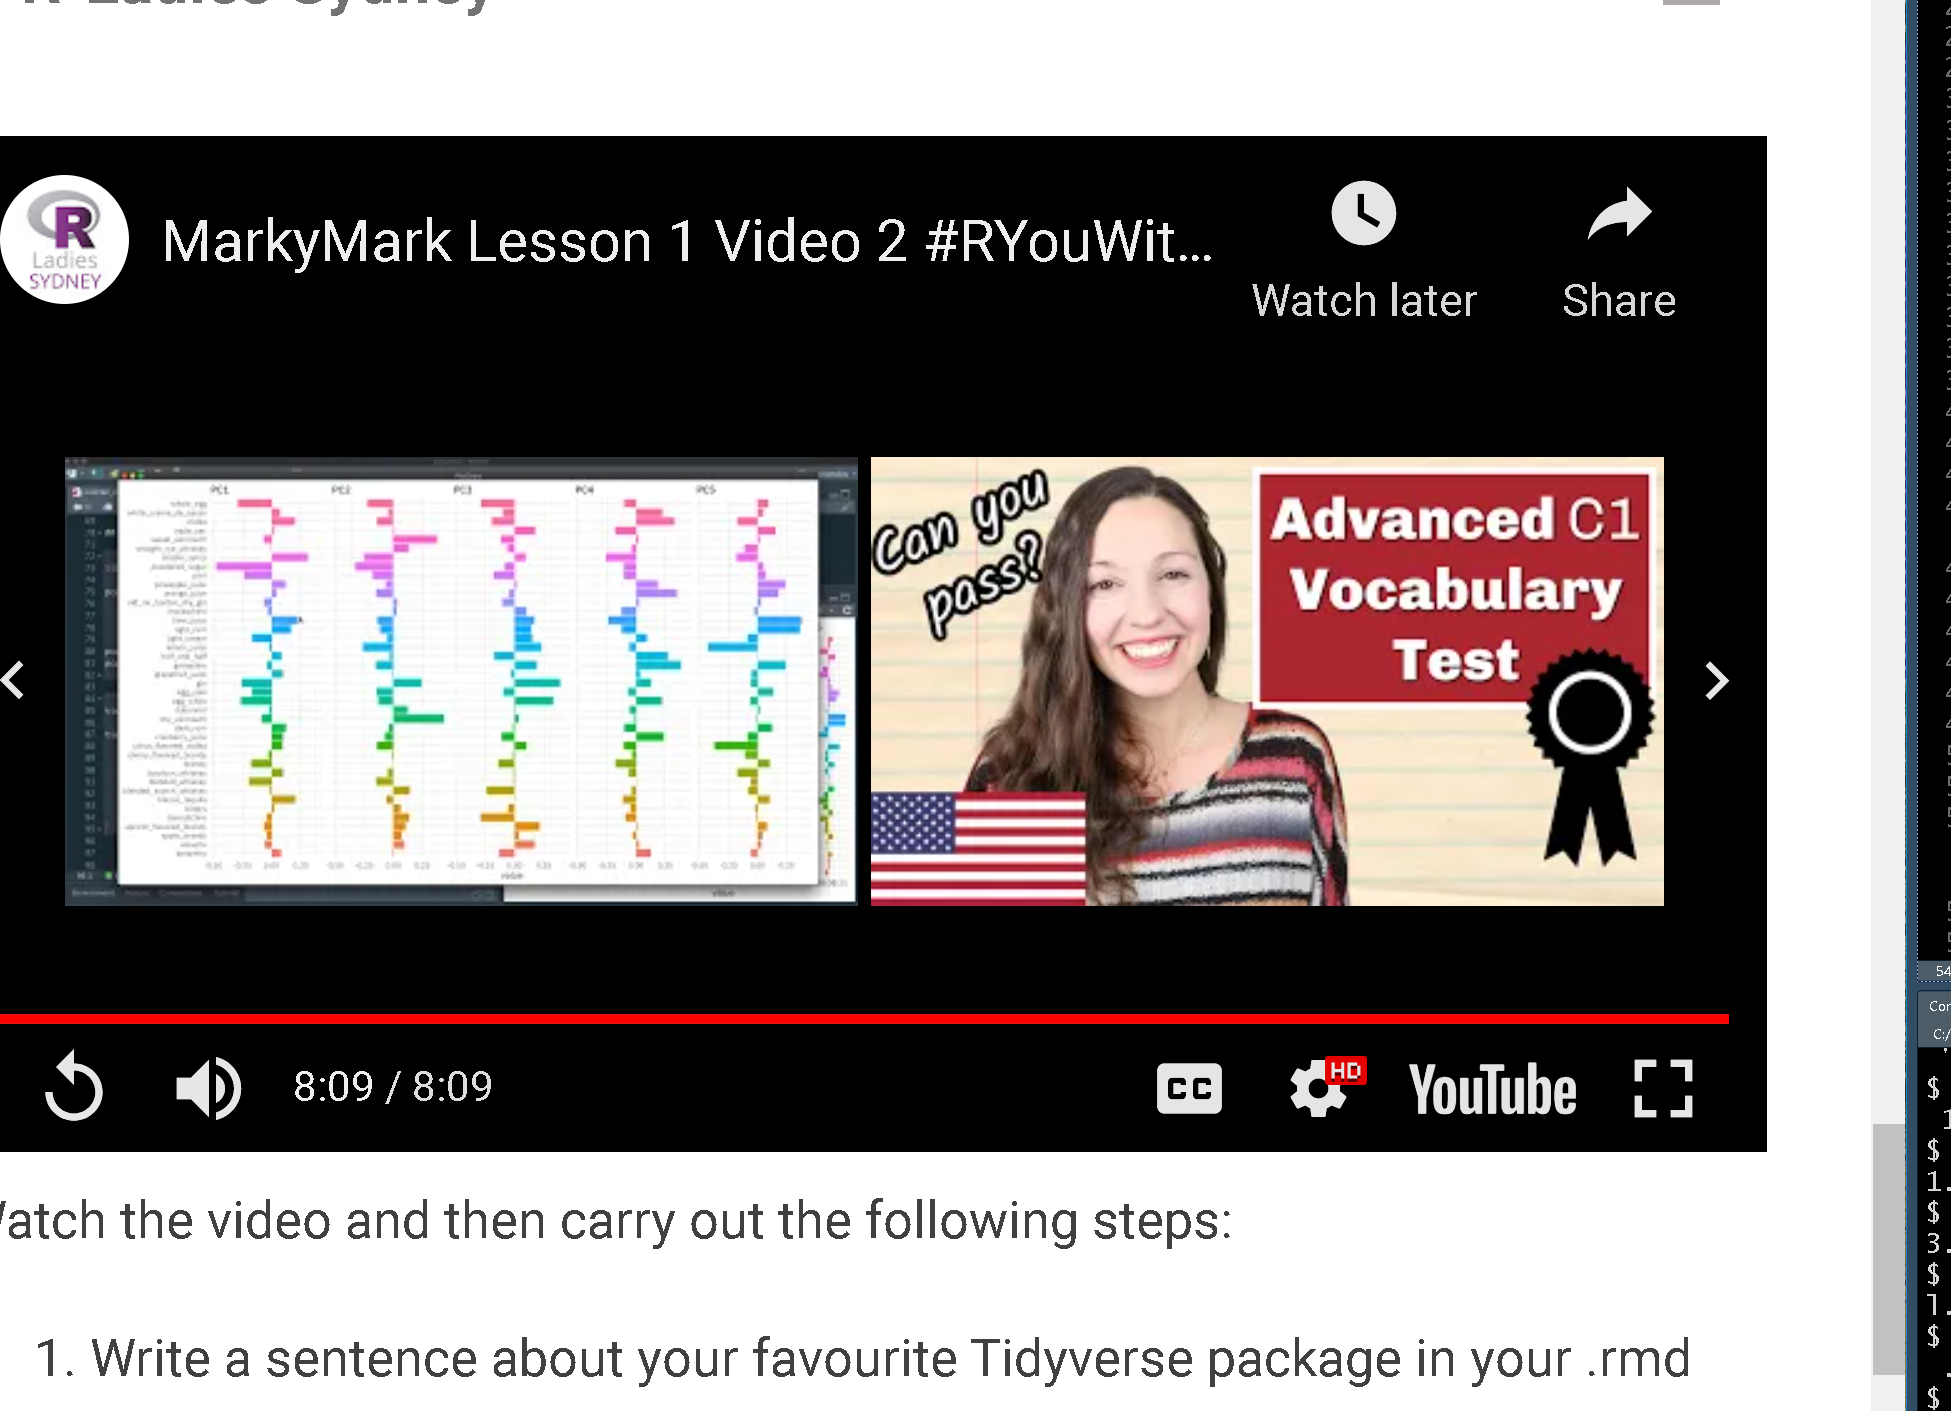
\includegraphics{markymarktestimage.png}
\caption{text to explain image}
\end{figure}

\hypertarget{tweetsgifsother-media}{%
\subsubsection{tweets/gifs/other media}\label{tweetsgifsother-media}}

copy and paste the embed code from the media website into your markdown
report

use single tick mark around
\texttt{text{[}{]}if\ you\ want\ it\ printed\ as\ a\ command}

\hypertarget{insert-code}{%
\section{insert code}\label{insert-code}}

to power of markdown is that you can insert and execute code chucks, and
control what output does or does not appear in the final report. - to
insert a code chunk use button at top or keyboard shortcut ctrl+ alt+I -
to execute code chunk press green arrow at end of chunk or ctrl+enter -
to control what output appears in your report add parameters to \{r\}

\hypertarget{load-pkgs}{%
\paragraph{load pkgs}\label{load-pkgs}}

if some of output is included (can add warnings and more verbose output
to report)

\begin{Shaded}
\begin{Highlighting}[]
\FunctionTok{library}\NormalTok{(tidyverse)}
\end{Highlighting}
\end{Shaded}

\begin{verbatim}
## -- Attaching packages --------------------------------------- tidyverse 1.3.0 --
\end{verbatim}

\begin{verbatim}
## v ggplot2 3.3.3     v purrr   0.3.4
## v tibble  3.0.5     v dplyr   1.0.3
## v tidyr   1.1.2     v stringr 1.4.0
## v readr   1.4.0     v forcats 0.5.1
\end{verbatim}

\begin{verbatim}
## -- Conflicts ------------------------------------------ tidyverse_conflicts() --
## x dplyr::filter() masks stats::filter()
## x dplyr::lag()    masks stats::lag()
\end{verbatim}

if all output is removed from showing up in your report

\begin{Shaded}
\begin{Highlighting}[]
\FunctionTok{library}\NormalTok{(readr)}
\FunctionTok{library}\NormalTok{(here)}
\end{Highlighting}
\end{Shaded}

\hypertarget{read-in-data}{%
\paragraph{read in data}\label{read-in-data}}

\begin{Shaded}
\begin{Highlighting}[]
\NormalTok{beaches }\OtherTok{\textless{}{-}} \FunctionTok{read.csv}\NormalTok{(}\FunctionTok{here}\NormalTok{(}\StringTok{"Data"}\NormalTok{, }\StringTok{"cleanbeaches.csv"}\NormalTok{))}
\end{Highlighting}
\end{Shaded}

\hypertarget{plot-mean-number-of-bugs-at-each-beach}{%
\paragraph{plot mean number of bugs at each
beach}\label{plot-mean-number-of-bugs-at-each-beach}}

\begin{Shaded}
\begin{Highlighting}[]
\NormalTok{beaches }\SpecialCharTok{\%\textgreater{}\%} 
  \FunctionTok{group\_by}\NormalTok{(site) }\SpecialCharTok{\%\textgreater{}\%} 
  \FunctionTok{summarise}\NormalTok{(}\AttributeTok{meanbugs =} \FunctionTok{mean}\NormalTok{(beachbugs, }\AttributeTok{na.rm =} \ConstantTok{TRUE}\NormalTok{)) }\SpecialCharTok{\%\textgreater{}\%} 
  \FunctionTok{ggplot}\NormalTok{(}\FunctionTok{aes}\NormalTok{(}\AttributeTok{x =}\NormalTok{ site, }\AttributeTok{y =}\NormalTok{ meanbugs)) }\SpecialCharTok{+}
  \FunctionTok{geom\_col}\NormalTok{() }\SpecialCharTok{+}
  \FunctionTok{coord\_flip}\NormalTok{()}
\end{Highlighting}
\end{Shaded}

\includegraphics{markyMark_files/figure-latex/unnamed-chunk-3-1.pdf}

\hypertarget{other-export-formats}{%
\section{other export formats}\label{other-export-formats}}

by default your markdown report will export as html, but you can also
choose to export as word doc or pdf by clicking down arrow next to knit
button and changing the output specified in your header.

\hypertarget{word}{%
\paragraph{word}\label{word}}

if you knit to word, your report will launch ms word in separate window
and open your doc.

\hypertarget{pdf}{%
\paragraph{pdf}\label{pdf}}

can be finniky, at times won't produce pdf. works with latex. so if it
doesn't work may be to install and load the ``tinytex'' pkg.

\begin{Shaded}
\begin{Highlighting}[]
\FunctionTok{library}\NormalTok{(tinytex)}
\end{Highlighting}
\end{Shaded}

i installed and loaded tinytex, but still couldn't get pdf report to
knit successfully.

here is screenshot of the error message
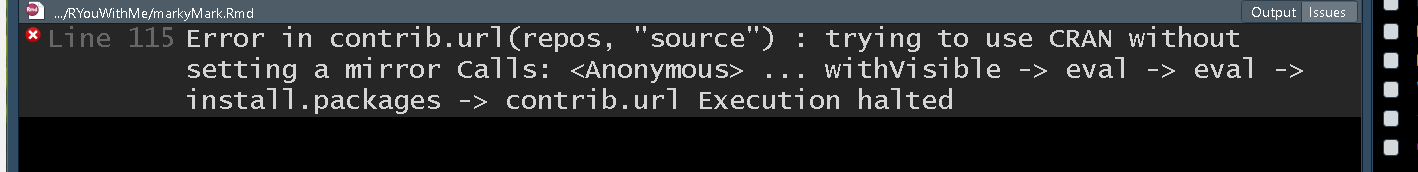
\includegraphics{knit_pdf_error.png}

\end{document}
